\section{Questions sur le chapitre ``Machine de détente''}
\subsection{Que représente le rendement polytropique interne d'une machine réceptrice ?}
Le rendement polytropique permet de modéliser les travaux de frottement. Pour une machine réceptrice où on néglige les termes d'énergie cinétique et de gravité, on a :
\begin{equation} w_m = \int vdp + w_f = \frac{\int vdp}{\eta_{Pi}} \end{equation}
En modélisant $w_f = \alpha w_m$, on peut facilement trouver que $\alpha = 1-\eta_{Pi}$. Formulé autrement :
\begin{equation} \eta_{Pi} = \frac{w_m-w_f}{w_m} = \frac{\int vdp}{w_m} \end{equation}
Le rendement polytropique représente donc le rapport du travail utile sur le travail fourni.

\subsection{Rendement isentropique et polytropique d'une turbine : lequel est le plus grand ? Justifiez à l'aide d'un graphe.}
On sait que dans le cas d'une turbine, on a 
\begin{equation} \eta_{Si} = \frac{h_a-h_e}{h_a-h_{es}} \end{equation}
Sur la Figure \ref{fig:isenpoly}, on peut voir que l'enthalpie du point $a$ est la même que celle du point $a'$ car elle ne dépend que de la température. Le rendement isentropique est donc égal au rapport de la région rose sur la somme des régions rose et rouge. 
Le rendement polytropique quant à lui est égal au rapport de la région rose sur la somme des trois régions. Le rendement polytropique est donc plus petit que le rendement isenthalpique dans le cas d'une turbine. 
\begin{figure}[h]\centering
	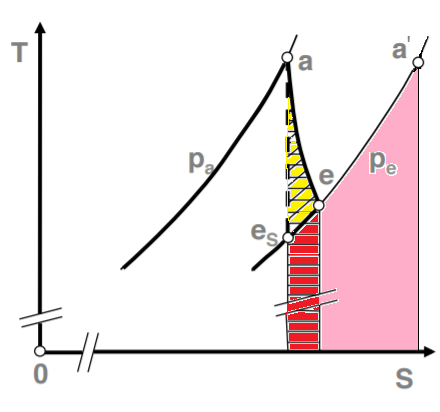
\includegraphics[width=0.5\textwidth]{figures/isenpoly.png}
	\caption{Détente isentropique et polytropique.}
	\label{fig:isenpoly}
\end{figure}
